% The following choice requires a coordinated choice when PRINTING the report:
%\documentclass[oneside,12pt]{report}  % Use this for one-sided copying (print with printer's normal
%  single-sided option
\documentclass[twoside,12pt,openright]{report}  % You can use this for a slim final printed copy (print with 
%  printer's double-sided option)

% the dimensions of the page
\textheight=9.25in \topmargin=-0.5in   %See note in Chapter 8 of Sample Report about "Page scaling" option in Adobe
\textwidth=6.0in
\oddsidemargin=0.3in
\evensidemargin=0.3in  % Needed to balance even and odd pages in twoside print copy

% Useful packages
\usepackage{amsmath}
\usepackage{amsfonts}
%% In the following, the assumption is that your graphics are in encapsulated postscript (eps).  If not,
%% you may need to use some other method for incorporating graphics into your pdf of the final report.
%  Use the next package for typesetting directly to dvi or postcript (used primarily for the PCTeX typesetter, 
%  see the following alternatives).
\usepackage[dvips]{graphicx} 
% Use the next two packages together for typesetting directly to pdf (this works for pdfLaTeX and may work 
% for others---not yet tested for all---please report your experience).
%\usepackage[pdftex]{graphicx}
%\usepackage{epstopdf}
%%

\usepackage{doc}
% Following sets up logic and formatting for conditional twoside copying
\usepackage{ifthen, color, fancyvrb}
\usepackage{nextpage}\pagestyle{plain}
\newcommand\myclearpage{\cleartooddpage
  [\thispagestyle{empty}]
  }

%  Set font size for captions
\usepackage[skip=4pt,font=footnotesize]{caption}


\DeclareGraphicsExtensions{ps,eps}
\usepackage{excludeonly}

% If some words are being hyphenated incorrectly, they can be
% given in a list to the \hyphenation command as below.
\hyphenation{ap-pen-dix wer-ther-i-an}

% Theorem-like command definitions:
\newtheorem{theorem}{Theorem}[chapter]
\newtheorem{lemma}{Lemma}[chapter]
\newtheorem{definition}{Definition}  % Note, this italicizes everything

% Print the chapter and sections in the toc
\setcounter{tocdepth}{1}

% Specify which files to typeset for this run (note that overall pagination is preserved)
%\includeonly{chapter1, chapter2}

% Specify which files NOT to typeset for this run (note that overall pagination is preserved)
%\excludeonly{}

% Groundwork for allowing double-sided copying with blank versos
\def\prefacesection#1{
\chapter*{#1}
\addcontentsline{toc}{chapter}{#1}
}

\begin{document}

% Footnote references are symbolized in the front matter, but see below for restoration of numbered footnotes in the body.
\def\thefootnote{\fnsymbol{footnote}}

% The title page is in its own file, ``titlepage.tex''.
% It needs to be edited to reflect information specific
% to your project. 
% don't display the page number
\thispagestyle{empty}

% The numbers below controls the amount of space between the following sections
\def\shiftdowna{0.32in}  % Adjust for balance
\def\shiftdownb{0.22in}  % Adjust for balance

% Set up the boiler plate at the top of the page

\begin{center}
\textbf{{\large Summer Research Program in Industrial \\ and Applied Mathematics}}\\

\vspace \shiftdowna
%\includegraphics[width=0.4\textwidth]{ipam.eps}\\

\begin{figure}[h]
  \centering
  \begin{minipage}[b]{0.4\textwidth}
    \centering
    \includegraphics[width=3cm]{Graphics/HKUST_logo.jpg}
      \end{minipage}
 % \hfill
  \begin{minipage}[b]{0.4\textwidth}
    \centering
    \includegraphics[width=6cm]{Graphics/SNU_logo.jpg}
      \end{minipage}
\end{figure}

% SPONSOR
\vspace \shiftdowna
\underline {Sponsor}\\ 
\vspace{5pt}
$\langle \textbf{{\large Magnum Research Limited}} \rangle$ \\
\vspace \shiftdowna
\textbf{Final Report}

% TITLE
\vspace \shiftdowna
$\langle \textbf{{\Large Portfolio Management using Reinforcement Learning}}\rangle$

% Note the convention used here:  email addresses and urls are typeset in teletype font, colleges are set in italics.

% STUDENTS
\vspace{0.35in}
\underline {Student Members}\\
\vspace{5pt}
$\langle \text{SEO Dayoung}\rangle$ (Project Manager), $\langle \text{\emph{SNU}}\rangle$,\\ 
\vspace{3pt}
$\langle \text{\texttt{multiply@snu.ac.kr}} \rangle$\\
\vspace{5pt}
$\langle \text{PARK Junggil}\rangle$, $\langle \text{\emph{SNU}} \rangle$ \\
\vspace{3pt}
$\langle \text{WONG Singlam}\rangle$, $\langle \text{\emph{HKUST}} \rangle$ \\
\vspace{3pt}
$\langle \text{YANG Yuwei}\rangle$, $\langle \text{\emph{CityU HK}} \rangle$ \\

% ACADEMIC MENTORS
\vspace \shiftdownb
\underline {Academic Mentor} \\
\vspace{5pt}
$\langle \text{Avery Ching}\rangle$, $\langle \text{\texttt{maaching@ust.hk}} \rangle$

% SPONSORS
\vspace \shiftdownb
\underline {Sponsoring Mentors}\\
\vspace{5pt}
$\langle \text{Joseph Chen}\rangle$, $\langle \text{\texttt{joseph.chen@magnumwm.com}} \rangle$\\
$\langle \text{Don Huang}\rangle$, $\langle \text{\texttt{Contact Info}} \rangle$
\vspace{3pt}



% DATE
\vspace \shiftdowna
$\langle \text{Date: August 8, 2018}\rangle$ 

\end{center}

%\vfill  %Fill page to force following note to bottom
%\footnoterule
%\noindent \small{This project was jointly supported by HKUST and SNU.} 



% Begin ABSTRACT
\ifthenelse{\boolean{@twoside}}{\myclearpage}{}
\prefacesection{Abstract}
% don't display the page number
%\thispagestyle{empty}

In this project, we use Q-learning and deep Q-network to train agents that manage a stock portfolio of two stocks. We defined a state as the stock price change history, and an action as the weight between two stocks, and a reward as portfolio value change or sharpe ratio. In most cases Q-table or neural networks performed better than the 50-50 reevaluate benchmark when we trained, but when we use Q-table and neural networks to test on unknown datasets, they are not good as the benchmark.	


% Begin ACKNOWLEDGMENTS
\ifthenelse{\boolean{@twoside}}{\myclearpage}{}
\prefacesection{Acknowledgments}
We are  highly indebted to Dr. CHING Avery, Dr. CHEN Joseph and Dr. HUANG Don for their guidance and constant supervision as well as for providing necessary information regarding the project. Thanks Dr. KU Albert Yin-Bon, Proof. LEUNG Shing-Yu and Dr. KOOK Wong to hold this meaningful program and the support from Mathematics Department of HKUST and SNU in completing the project.




% Table of contents, List of Figures, and List of Tables.
\ifthenelse{\boolean{@twoside}}{\myclearpage}{}
\tableofcontents

\ifthenelse{\boolean{@twoside}}{\myclearpage}{}
\listoffigures

\ifthenelse{\boolean{@twoside}}{\myclearpage}{}
\listoftables

% The report is an extensive document.
% It is convenient to have each chapter of the report in its own file
% rather than throw all work together in a single file.
% Do not run the LaTeX typesetter on each individual chapter; refresh
% your report by running the typesetter on this master file.

% Cancel the previous symbol requirement for footnotes in the front
% matter, and use arabic numerals for footnotes in the body
\renewcommand{\thefootnote}{\arabic{footnote}}
\setcounter{footnote}{0}

% Chapter 1 -- the Introduction
\ifthenelse{\boolean{@twoside}}{\myclearpage}{}
\chapter{Introduction}\label{Ch:Introduction}

The introduction should describe what the purpose of the project is/was and what you have accomplished.
The introduction, as well as other parts of the report, can be developed incrementally and will evolve with the project.
The introduction should contain the following items:
\begin{enumerate}{}
\item a brief description of the sponsoring organization (which often can be derived from the organization's online boilerplate), 
\item a suitably condensed statement of the problem posed by the sponsor, 
\item some discussion of the relevance of the project to the sponsor's business, 
\item the team's approach to the problem, gleaned from the team's Work Statement (including a summary of background study, i.e., literature review, to explain how your work differs from or builds on previous efforts --- this explanation should be reinforced by entries with annotation in the bibliography),
\item summary of the report: in separate paragraphs specify and summarize the major sections of your report (Ch 2, Ch 3, ... , Conclusion,  Appendixes, Glossary, Bibliography).
\end{enumerate}

The team as a whole is responsible for the development of a RIPS report, but various aspects will be divided among individuals, as your team will choose.
A Report Coordinator (RC), selected from the team in the first week of the project, will be responsible for incorporating evolving components of your team's report into the {\LaTeX} template that was used to typeset this document, produced in a particular style we refer to as the {\it RIPS  House Style}.

The template requires familiarity, and so a {\LaTeX} tutorial explaining its use  will be given during the second week of RIPS, and a special section for RCs is available in the ``Templates-etc'' folder on IPAM's R-Drive.
For more information, see  also the  README file.
Prior familiarity with {\LaTeX}  would be advantageous for an RC, but expertise is not necessary because assistance will be provided by RIPS.


\endinput


% Chapter 2
\ifthenelse{\boolean{@twoside}}{\myclearpage}{}
\chapter{Methodology for Q-learning and Deep Q Network}
\label{Ch:methodology}

The main methodologies we are using for the research are Q-Learning and Deep Q Network(DQN). Here are some explanations about those methodologies.

\section{Q-learning}
Q-Learning is one of the Reinforcement Learning algorithms that attempts to learn the value of being in a given state, and taking a specific action there. Q-table is a table of values for every state(row) and action(column) possible in the environment. Within each cell of the table, we learn a value for how good it is to take a given action within a given state.  We start by initializing the table to be all zeros, and then as we observe the rewards we obtain by taking various actions, we update the table accordingly.

When updating the Q-table, Bellman equation is used. Bellman equation’s concept is that the expected long-term reward for a given action in a given state is equal to the immediate reward gained from the current action plus the expected reward from the best future action taken at the following state. Q-table is used to estimate the long-term reward. As shown below, Q-value for a given state(s) and action(a) should equal to the current reward(r) plus the maximum discounted($\lambda$) future reward expected according to Q-table for the next state$(s’)$ we would end up in. 
$$Q(s,a) = r + \lambda (\max (Q(s’,a’))$$

In Q-learning, for every training process, we first check whether the state already exists in the q-learning table, if it exists, we choose the action with the largest Q-value. If it doesn’t exist, we build a new empty line of this state and random choose action. Then we update the value in the q-learning table by  Q-TABLE learning formula .

As we use q-learning model, we need to discretize the states and actions. For actions, we discretize it by choosing actions as the weight of stock A of the total portfolio value and only keep one decimal. So we define the action vector as $(0, 0.1, 0.2, …, 0.9, 1)$. For the states, we tried two models. We first use the pair of stocks’ close price, but it is not general enough to be used as states in q-learning model. Then we generalize the states by using the pair of stocks’ close price change, and only keep two decimals. After that, we generalize our states by using another method. We using the slopes of the linear regression functions of the stocks’ each fixed period(3 days, 10 days).

For the reward function, at the first we simply used portfolio value change as a reward. However, as for portfolio management, we should not only consider the profit, but the risk. Thus we use sharpe ratio as the model’s reward function. Sharpe ratio formula 

\subsection{Q-learning Algorithm}
\def\skipl{0.2in}
\vspace{\skipl}
\fbox{
\begin{minipage}{5in}
Initialising $Q(s,a)$ arbitrarily 

Repeat (for each episode):

Initialise $s$

Repeat (for each step of a episode):

Choose $a$ from $s$ using policy derived from $Q$ (e.g. $\epsilon$ greedy)

Take action $a$, observe $r$, $s’$
\begin{equation}\label{eq:q-update}
Q(s,a) \leftarrow Q(s,a)+\alpha (r+\gamma \max_{a'} Q(s',a')-Q(s,a))
\end{equation}
\begin{equation}\label{eq:s-update}
 s \leftarrow s'
\end{equation}
Equation \eqref{eq:q-update} and \eqref{eq:s-update} are the update equations.
\end{minipage}}
\vspace{\skipl}

\section{Deep Q Network (DQN)}
Deep Q Network uses the techniques from deep learning to approximates Q-score, since in Q-Learning both state and action state need to be discrete and calculating and optimizing Q-score is both time and memory consuming. The key is that we apply the deep neural network to approximate the Q-function. We know that neural network is used to find out the right weights by the back propagation process so it can be used to map all state-action pairs to rewards. One standard example for neural network is using the convolutional neural network (CNN). 

Due to the problem of correlation between states and non-stationary targets, when we train the neural network, we store transition in memory M, and randomly sample mini-batch from M and replay to solve the problem. Plus, we separate the target network and copy the network regularly to solve non-stationary targets problem. Do a Forward Pass to get all possible Q values from the current state $s_t$.
\begin{enumerate}{}
\item Do a Forward Pass to get new state $s_{t+1}$ and argmax $a_{t+1}$. (Action that give us biggest Q-value)
\item Set Q-value target to $r+\gamma  \max Q(s',a')$ where $r$ is the reward and $\gamma$ is the discount rate.
\item Then use the backpropagation and stochastic gradient descent to update the network.
\end{enumerate}

Since CNN is a regression process, then the loss function will be squared.
$$L(\theta )=\frac{1}{2} \Big( R(s,a,a')+\gamma  \max Q(s',a';\theta)-Q(s,a;\theta) \Big)^2$$
\subsection{Algorithm}
\begin{figure}[H]
\begin{center}
\includegraphics[clip, width=1\textwidth]{Graphics/DQN.png} \caption{Deep Q-Network algorithm}
\end{center}
\end{figure}

% Chapter 3
\ifthenelse{\boolean{@twoside}}{\myclearpage}{}
\chapter{Data Description}
\label{Ch:figures}

The algorithms will be tested on stock market data or cryptocurrency data. For stock data, we will collect stock history of each day’s open price and close price by using Python library Pandas.DataReader. The stock history that we will use for training algorithm is from  2006.6.29 to 2018.6.29 which includes the financial crisis to train the model on non-occasional circumstances. 

Stocks are chosen among S \& P 500, considering the beta index, duration, and whether they contain some meaningful abrupt price change history. Samples we have chosen are from the top 10 stocks with the highest weight in S \& P 500’s high-beta index fund . 
\begin{table}[h]
\begin{center}
\begin{tabular}{|p{2in}|p{1in}|p{2in}|} \hline
Constituent & Symbol & Sector \\ \hline
Align Technology Inc  & BALGN & Health Care\\ \hline
Micron Technology Inc & MU & Semiconductor  \\ \hline
Nvidia Corp & NVDA & Semiconductor  \\ \hline
Lam Research Corp & LRCX & Semiconductor  \\ \hline
Advanced Micro Devices & AMD & Semiconductor  \\ \hline
NetFlix Inc & NFLX & Consumer Discretionary \\ \hline
Applied Materials Inc & AMAT & Semiconductor \\ \hline
KLA-Tencor Corporation & KLAC & Semiconductor / Material \\ \hline
Freeport-McMoRan Inc & FCX & Mining and Metal \\ \hline
Incyte Corp & INCY & Health Care / Pharmaceutical  \\ \hline
\end{tabular}
\caption{Stock Data we used}\label{TABLE:SplitText}
\end{center}
\end{table}

We choose one stock from 10 high-beta stocks shown above, and another from low-beta stocks to make up our portfolio. In later steps, we choose K number of stocks considering the sectors, plus other foreign companies such as Lotte from South Korea to make the impact of exchange rate into consideration.



% Chapter 4
\ifthenelse{\boolean{@twoside}}{\myclearpage}{}
\chapter{Sample figures and tables}\label{Ch:figures}

\section{Figures}

% Note that the label follows the caption.
\begin{figure}[ht]
\begin{center}
\includegraphics[width=0.3\textwidth]{Graphics/ipamlogo.eps}
\end{center}
\caption{A sample \textsc{eps} figure with a caption.}\label{FIGURE:IPAM-logo-eps}
\end{figure} 


\subsubsection{Formats accepted by {\LaTeX}}
This version of the  RIPS {\LaTeX } template can be used to produce a pdf of your report using several different typesetters, including \texttt{pcTeX} and other options available on the IPAM network.
All of these will accept figures in the encapsulated postscript (\textsc{eps}) format providing you incorporate the appropriate \emph{packages} in the \emph{preamble} of your {\LaTeX] code.%%
\footnote{
The RIPS reports template devotes a section of the preamble to a method for ensuring that your chosen typesetter will be able to utilize eps files. 
This is one of several options for affecting formats that you will find explained by comments in the preamble.
For a good source for general information on incorporating graphics in {\LaTeX}, see
\texttt{http://amath.colorado.edu/documentation/LaTeX/reference/figures.html}.
}%% 
The LaTeX code for Figure \ref{FIGURE:IPAM-logo-eps} shows how to emplace, label and reference it.
You may have to convert the format for your figure.
But beware, incorporating graphics in {\LaTeX} can be quirky and require special attention and work-arounds.%%
\footnote{There is a simple way to make format conversions that works in some cases.
Click on the file in its current format, then when the graphic appears on your screen use ``save as'' to write the graphic in a format you select from the given options.
See Chapter 7 for more suggestions.}

\subsubsection{Creating figures with {\textsc{Matlab}}}
Here's a sample code, describing how to create a figure in \textsc{Matlab} and export it as \textsc{eps}.

\begin{verbatim}
%% Shows how to make a MATLAB figure

%% create a vector of N points between a and b
a=-1.2; b = -a; N = 100; X=linspace(a, b, N);

Y = X.^3 - X; % a function of X

figure(1); clf; % pop up a figure, clean it

H = axes; set(H, 'fontsize', 20); % set the font

plot(X, Y, 'color', 'blue', 'linewidth', 2); % plot

axis([a, b, -0.6, 0.6]); % the viewable box

saveas(gcf, 'MyPicture.eps', 'psc2'); % save the picture in color
\end{verbatim}

\begin{figure}[h]
\begin{center}
\includegraphics[clip, width=0.4\textwidth]{Graphics/MatlabPicture.eps}
\caption[A sample figure created as an \texttt{eps} file by \textsc{Matlab}]{A sample figure created as an \texttt{eps} file by \textsc{Matlab}.
To see an example of quirky treatment, compare this figure when you typeset the report template with \textsc{PCTeX} and pdf{\LaTeX}.}\label{FIGURE:fromMatlab}
\end{center}
\end{figure}

The source code for Figure \ref{FIGURE:fromInkScape} is available in the sample RIPS report directory. 
The {\LaTeX}code for incorporating this figure in the report template is:

\vspace{8pt}
\begin{quote} 
{\tt $\backslash$begin\{figure\}[h]\\
{\tt $\backslash$begin\{center\}} \\
{\tt $\backslash$includegraphics[clip, width=0.4$\backslash$textwidth]{Graphics/MatlabPicture.eps}} \\
{\tt $\backslash$caption\{A sample figure created with $\backslash$textsc\{Matlab\}.\}}$\backslash$label{<name of label}}  \\
{\tt $\backslash$end\{center\}} \\
{\tt $\backslash$end\{figure\}}
\end{quote}

Beware: your label identifier should always follow the caption statement.
You can place it higher up without crashing the {\LaTeX} compiler, but doing so can result in an erroneous enumeration for the label in your text.

\subsubsection{Software for drawing diagrams}

There exist many programs for drawing figures and diagrams.
If you have a preferred system, please let the RIPS director know about it.
Maybe it should be referenced here.
The following two were recommended by Academic Mentors:

\textsc{PSTricks} is a powerful system for designing and incorporating fine mathematical graphics into {\TeX} and {\LaTeX} documents.
Be aware that it works directly with inline code for some {\LaTeX} typesetters but  requires special handling for pdf{\LaTeX}.  
See Figure \ref{FIGURE:fromPSTricks}.


\begin{figure}[h]
\begin{center}
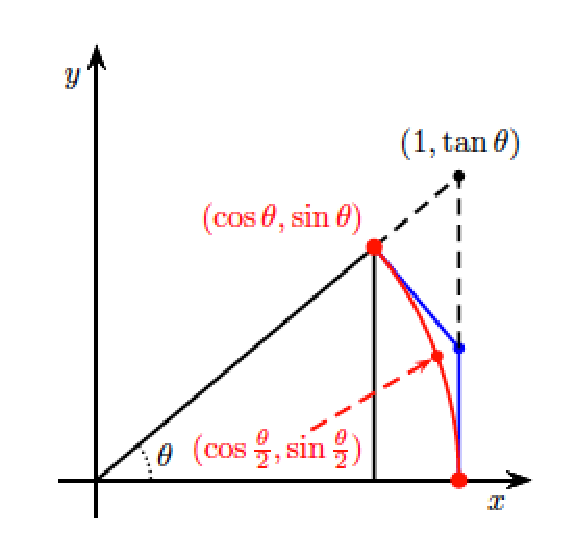
\includegraphics[clip, width=0.4\textwidth]{Graphics/SineTheta5-CS.eps}
\caption[A sample figure created as an \texttt{eps} file by \textsc{Matlab}]{PSTricks code for this figure is in the ``Graphics'' folder for the {\LaTeX} template.
The code was run using Xe{\LaTeX} and the resulting \texttt{pdf} file was converted to an \texttt{eps} file.}\label{FIGURE:fromPSTricks}
\end{center}
\end{figure}


\emph{Inkscape} is free and of high quality;
with this program, you should always keep the figures in Inkscape's native \textsc{svg} format,
and save them as \textsc{eps} only in order to view them in {\LaTeX}.


\begin{figure}[ht]
\label{fig2}
\begin{center}
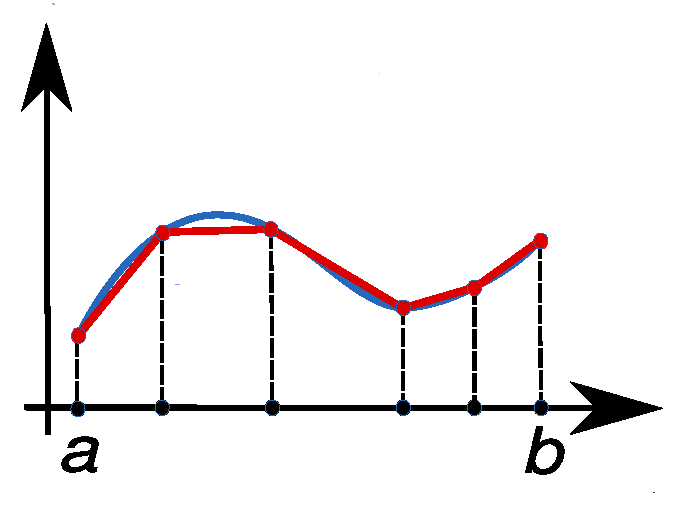
\includegraphics[width=0.4\textwidth]{Graphics/Figure1.eps}
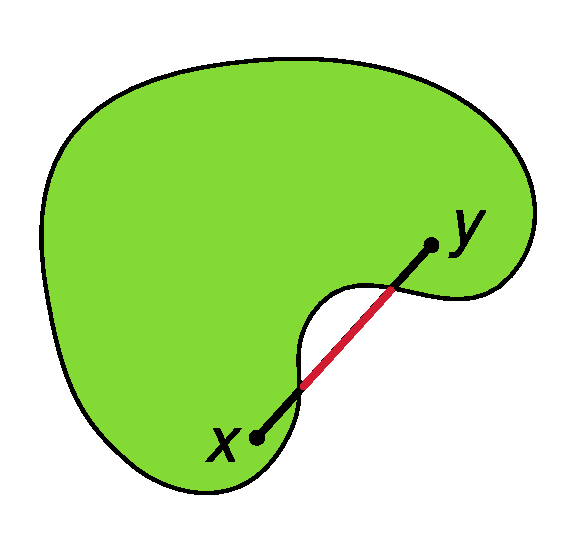
\includegraphics[width=0.309\textwidth]{Graphics/Figure2.eps}
\end{center}
\caption{A couple of figures drawn with Inkscape.}\label{FIGURE:fromInkScape}
\end{figure}

The two adjacent graphics in Figure \ref{FIGURE:fromInkScape} were created with Inkscape and exported to \textsc{eps}.
The figures in the original \textsc{svg} format are available in the report directory.
Note that the convention for punctuating a figure caption or table caption is pretty loose.
If an initial phrase is followed by a complete sentence, the phrase as well as any complete sentence should be ended with a period.
For consistency, it is \textsc{ok} to end all captions with a period even if a caption is just a phrase, as are all three captions illustrated here.

\section{Tables}

\noindent The next example is a simple table: Table \ref{TABLE:Simple}.
The {\LaTeX} code for it is presented after the table. 

% Note that the label follows the caption.
\begin{table}[h]
\begin{center}
  \begin{tabular}{|lcc|}
    \hline
    Date & High & Low\\ \hline
    1-Jul & 40 & 12\\
    2-Jul & 37 & 14\\
    3-Jul & 35 & 20\\ \hline
  \end{tabular}
\end{center}
\caption{A simple table showing fictional data.}\label{TABLE:Simple}
\end{table}

Look at the following source code for Table \ref{TABLE:Simple}, and note particularly how it is labeled.
The references to it in the two preceding sentencs were created by incorporating the label in the {\LaTeX} code 
(``\verb+Table \ref{TABLE:Simple}+'') used for creating this chapter.
Tables are labeled and referenced in a way similar to figures.

\begin{verbatim}
% Note that the label follows the caption.
\begin{table}[h]
\begin{center}
  \begin{tabular}{|lcc|}
    \hline
    Date & High & Low\\ \hline
    1-Jul & 40 & 12\\
    2-Jul & 37 & 14\\
    3-Jul & 35 & 20\\ \hline
  \end{tabular}
\end{center}
\caption{A sample table showing fictional data.}\label{TABLE:Simple}
\end{table}
\end{verbatim}

The next example, Table \ref{TABLE:SplitText}, illustrates a table in which column widths are specified by parameters in order to force long text to be spread over more than one line: 

\begin{table}[h]
\begin{center}
\begin{tabular}{|p{1in}|p{2in}|} \hline
Betty & Betty has a story to tell. \\ \hline
Bob   & Bob has a longer story to tell. \\ \hline
Bill  & Bill has a very much longer and far more dramatic story to tell. \\ \hline
\end{tabular}
\caption{A sample table with split lines of text.}\label{TABLE:SplitText}
\end{center}
\end{table}

\noindent Here's the code for Table \ref{TABLE:SplitText}:

\begin{verbatim}
\begin{table}[h]
\begin{center}
\begin{tabular}{|p{1in}|p{2in}|} \hline
Betty & Betty has a story to tell. \\ \hline
Bob   & Bob has a longer story to tell. \\ \hline
Bill  & Bill has a very much longer and far more dramatic story to tell. \\ \hline
\end{tabular}
\caption{A sample table with split lines of text.}\label{TABLE:SplitText}
\end{center}
\end{table}
\end{verbatim}

\subsubsection{Style tips about figures and tables}
You should always make sure that your figures are easy to see, so for example, make sure that any curves are not too thin or text is not too small.
And don't forget to include axis labels with units specified.

Your figures should look good both in color and as black-and-white, since for presentations you will most likely want figures in color, while in a printed report all the figures will usually be printed in black-and-white (and then, what looks very clear and pretty on your screen may appear as a dark region on paper).

Good captions greatly improve the usefulness of figures and tables.

But no matter how well a caption describes a figure or table, you should always reference it and explain it in your text.
You may feel you are being redundant, but your readers won't think so:
a picture with a good description is worth a thousand words, and a picture without a description in the text is left dangling.

\section{Picking nits}
Notice that in this sample report, all of the captions for figures and tables are placed below the object, and their labels end with a numbered identifier---e.g., Figure 4.1, Table 4.2---terminated with a colon (``:'') inserted automatically by the {\LaTeX} compiler. 
\emph{The Chicago Manual of Style} specifies the use of a period (``.'') to follow the figure number and a blank space to follow the table number, and \emph{New Hart's Rules} follows both figure and table numbers with a blank space.  
Moreover, \emph{New Hart's Rules} places table captions above the table, rather than beneath.
But here we bow to usage in {Gr\"{a}tzer's} \emph{More Math Into {\LaTeX}}(See Bibliography for references).
In such minutiae it's your choice, but remember, consistency (perhaps a hobgoblin of lesser minds but certainly a ruling passion in typography) is standard practice. 


Another place to be on guard is in referencing, e.g., sections, equations, and lemmas.
Do you capitalize or leave it in lower case: Chapter 1 or chapter 1, Theorem 1 or theorem 1, Lemma 1 or lemma 1?
Of course at sentence heads you have no choice but to capitalize.
When you refer to a figure or a table, you may write, for example, ``Fig. 1'', ``Figure 1'', with or without an initial capital, and write ``Table 1'' or ``table 1''.
Recommended usage for this report is to use proper nouns: whether abreviated or spelled out in full, capitalize the labels.
It's up to you, but be consistent.

You'll think of other things as you go along.
Just consider how it looks on the page, and {\it be consistent throughout your report}.

\endinput



% Chapter 5
\ifthenelse{\boolean{@twoside}}{\myclearpage}{}
\chapter{Dealing with bibliographic references}\label{Ch:References}


{\LaTeX} uses a tool called {\BibTeX} to help you manage bibliographic references.
The references are maintained in a separate file, with a \texttt{.bib}
extension. For example, in this sample RIPS report the references
are in the \texttt{Biblio.bib} file, which is then included
from the main document.

{\BibTeX} affords a variety of \emph{entry types} (also known as \emph{record types}) for bibliographic records of books, articles, proceedings, theses, and many others.  
A good discussion of these and of the \emph{field entries} used for each type, find the \textsc{Wikipedia} article for {\BibTeX}.
You can use any editor to create your own bibliographic records, but you might find useful open-source tools available on the web.%%
\footnote{
Appendix \ref{App:BibTeX-Records} lists some examples of record types and fields used for {\BibTeX} entries.
}
%%

If you would like to include a reference to a book or an article in the
{\BibTeX} file, you can either create its {\BibTeX} entry by hand, or get it 
ready-made as a BibTeX entry from a web source. 
\emph{Google Scholar}, which you can find on the internet, is free and easy to use after you have set up preferences to include citations in a {\BibTeX} format.
Ask your Academic Mentor for other suggestions.%%


After you update your report's references file, to see the updated
references displayed in the report you need to run {\LaTeX} on the
report, then run {\BibTeX} (on the report, not on the references
file), and then run {\LaTeX} on the report again, once or a couple
of times.%%
\footnote{
Some typesetters can operate in a mode that performs all these operations in the correct sequence automatically.
}
%%
Don't be surprised if it takes you awhile to get used to
this routine---you won't be the first. Look for the {\BibTeX} icon or \emph{Bibliography} tab
somewhere in your editor's toolbar.

For example, to cite the book \emph{More Math Into {\LaTeX}} by Gr\"{a}tzer \cite{gratzer}, first look in the \texttt{Biblio.bib} file to find that the entry for that reference is labeled \texttt{gratzer}.
Then enter the code \verb1\cite{gratzer}1 in your text.
After
\begin{itemize}
\item running {\LaTeX} on your document once,
\item then running {\BibTeX} on your document once,
\item then running {\LaTeX} on your document twice,
\end{itemize}
you will find the citation ``\cite{gratzer}'' obtained in the preceding paragraph, which is the correct number the reference for Gr\"{a}tzer's book winds up as in the Bibliography of this report.
Note that you do not run {\LaTeX} on the \texttt{.bib} file.

{\BibTeX} does take getting used to.
You may need some help from an experienced {\LaTeX}er when getting started.

\endinput


% Chapter 6
\ifthenelse{\boolean{@twoside}}{\myclearpage}{}
\chapter{Conclusion}
\label{Ch:Conclusion}


% Chapter 7
\ifthenelse{\boolean{@twoside}}{\myclearpage}{}
\chapter{Some extra advice for starting up with {\LaTeX}}\label{Ch:ExtraAdvice}

The following is a small collection of answers to questions RIPS students have asked.

\begin{enumerate}

%%%%
\item {\bf How do I open and modify {\LaTeX} files, as well as view the results?}
%%%%

Several {\LaTeX} typesetters are available on the IPAM network.
The default options are activated by clicking on the  main page for the report template,\\ 

\centerline{\texttt{z-Report-Master-2015.tex}}
\vspace{5pt}

The present version of the template is being maintained using the TeXworks typesetter "pdfLaTeX."
For more information about other options, see the  README file listed among the files used in construction this report.

\hspace{15pt} The template is divided into several chapters, appendixes and other files with functions identifiable by their names coded in {\LaTeX} (files ending in ``.tex'') along with some graphics files coded as Encapsulate Postscript (``.eps'').  
If you modify any one of these source files, you will need to run the typesetter on the main \texttt{z-Report-Master-2015.tex} file.
See Chapter \ref{Ch:References} for tips handling bibliographic references.
And see Appendix \ref{App:SourceLocation} for location of the {\LaTeX} sources relating to this sample report.

%%%%
\item {\bf Should I use a single-sided or double-sided format for my report?}
%%%%

Clearly, double-sided printing saves paper.
But this is not as simple as it seems.
Best to explain this in vocabulary used by publishers: {\em opening}, {\em recto}, and {\em verso}:
An {\em opening} is the pair of pages you see when you open a book at random; the recto is the page on the right-hand side, and the verso is the page on the left-hand side --- or, on a single leaf, recto is the front side and verso is the opposite side.
When you open almost any book at the start of a new chapter, the first page of the chapter will appear on the right-hand page---{\em recto}.
This is true whether or not the left-hand page of the opening---{\em verso}---is blank.
That's the way it should be in your report.
Each major section of your report, not just chapters, should begin on a recto.

\hspace{15pt} Rectos are always odd-numbered.
Very likely, you will not get these results if you submit your single-sided report for double-sided copying on a printer.
There are some {\LaTeX} acrobatics you must specify to make your double-sided report turn out with proper recto-verso pagination, the code for which is built into  \texttt{z-Report-Master-2014.tex};
you will see which document class to use---and which to comment out---at the top of the file.

%%%%
\item {\bf What format should I use for my report for the editing process, and for the final copies?}
%%%%

See Chapter \ref{Ch:Polishing}.

%%%%
\item {\bf How do I convert images (for example, in {\it \textsc{jpg}}, {\it \textsc{gif}}, {\it \textsc{bmp}}, or {\it \textsc{png}}   formats) to {\it \textsc{eps}}? }
%%%%

There is a simple procedure using a ``Terminal'' on an iMac: just invoke the ``\texttt{convert}'' command and specify the source and target file and coding.
Other methods can be complicated.

\hspace{15pt}Another possibility is to read them in \textsc{Matlab} and export them to \textsc{eps} from there.
Here's a sample code:

\begin{verbatim}
   A=imread('MyFigure.jpg');            % read the image
   imshow(A);                           % show it on the screen
   saveas(gcf, 'MyFigure.eps', 'psc2'); % export to color eps
\end{verbatim}

Note that this can create large \textsc{eps} files.
Simple diagrams are better recreated in \textsc{Inkscape} or \textsc{Matlab} and then exported to \textsc{eps}.

%%%%
\item {\bf What if a figure caption is too long to fit nicely in the list of figures?}
%%%%

Chapter \ref{Ch:figures} discusses figures in general;
there you can see an example of how a figure caption is created.
Ordinarily, the figure caption provides the text for the title for the figure in the report's List of Figures.

\hspace{15pt}But what if the figure caption is too long or otherwise inappropriate for using in the List of Figures?
The solution is to include an alternative title in square brackets (before the curly brackets---braces) in the caption declaration:

\begin{quote}
{\tt $\backslash$caption[Alternative title for List of Figures]\{The caption that appears under your figure; it can be more complex than is appropriate for a title in the List of Figures.\}}
\end{quote}

The same technique is used for providing alternative titles for tables---and for running heads as well, although these are not used in your RIPS report.

\item {\bf A useful little thing to know about fractions:} When you compose an inline fraction, sometimes it looks too small: $\frac{x}{y}$.  Instead of using the {\LaTeX} ``\texttt{frac}'' function, try ``\texttt{dfrac}'' to increase the size: $\dfrac{x}{y}$.

\item {\bf Where can I find more information on {\LaTeX}?}

The internet is a great resource.  Search and ye shall find! See, for example,\\

\centerline{$\texttt{http://latex-project.org/}$}
\vspace{5pt}

\hspace{15pt}Or you may want to get one of the books listed  in the Bibliography, for example, \emph{More Math Into {\LaTeX}} \cite{gratzer}, or the \emph{{\LaTeX}Companion} \cite{Mittelbach}.
Your mentor most likely knows a lot of {\LaTeX} too, so don't hesitate to ask for help.

%%%%
\item {\bf Where can I find standard references to resolve finer points of style?}
%%%%

There are many good references, but the RIPS director uses the $16^{\text{th}}$ edition of \emph{The Chicago Manual of Style} \cite{Chicago-Manual} and its companion \emph{A Manual for Writers of Research Papers, Theses, and Dissertations: Chicago Style for Students and Researchers} \cite{Turabian} as  references of first resort, followed by the handy compact reference \emph{Hart's New Rules} \cite{NewHartRules}.
Other highly developed style guides are the \emph{MLA Handbook for Writers of Research Papers} \cite{MLAHandbook} and the \emph{Publication Manual of the American Psychological Association} \cite{APA}.

\hspace{15pt}The examples in Gr\"{a}tzer's \emph{More Math into {LaTeX}} \cite{gratzer} can also be used to resolve some style questions as well as questions about {\LaTeX} coding.
See the bibliography pages for other good resources.

%%%%
\item {\bf How should I punctuate itemized and enumerated lists?}
%%%%

Here's a rule that gets broken easily because the items in a list are sometimes not just a single phrase or sentence.
Usually you will introduce your list with a sentence or phrase that ends with a colon.
In that case:

\begin{itemize}
\item begin each item with a lower-case initial letter;
\item terminate all but the last sentence with a semicolon or a phrase with a comma;
\item end the last sentence or phrase with a period.
\end{itemize}

\hspace{15pt}Here's an example that shows how any rule starts to get tricky:

\begin{itemize}
\item begin each item with a lower-case initial letter;
\item terminate the last sentence with a semicolon or a phrase with a comma,
\item but end the last sentence or phrase with a period.
\end{itemize}

\hspace{15pt}I think the comma at the end of the second item is correct, but you may be tempted to place a semicolon there to be consistent.
And in case you have more than one sentence, or a mixture of a sentence and a phrase on a single line, What then?
I'd prefer to avoid the latter complication if possible by make each item a simple sentence or phrase, and use only sentences or only phrases in a single list.

%%%%
\item {\bf Are there standard fonts for representing filenames, file extensions, URLs?}
%%%%

In this document we have used \texttt{teletype} for filenames and \textsc{small caps} for file extensions, program names, and the names of software packages.
For URLs, we use \texttt{teletype}.

%%%%
\item {\bf How do I write the {\tt tilde} symbol?}
%%%%

Just hitting the tilde   key on the keyboard won't work, as that
character is special to {\LaTeX}. Instead, use the \verb1\sim1
command, which gives $\sim$. The reason the plain keyboard tilde
character is special is that it is used for a non-breaking space,
e.g., by writing

\hspace{35pt} \verb+Dr.~Jones+

instead of simply

\hspace{35pt} \verb+Dr. Jones+

This is how to tell {\LaTeX} never to break a line after \verb+`Dr.'+ with
\verb+`Jones'+ starting at the beginning of the next line.

%%%%
\item {\bf {\LaTeX} and {\BibTeX} reserved characters}
%%%%

These characters are interpreted in special ways by {\LaTeX} typesetters: 
\vspace{5pt}

\centerline{\# \$ \% \^{} \& \_ \{ \} \~{} \textbackslash{}}

You may print them in your text by ``escaping'' them with the backslash (\textbackslash{}), e.g.,  use \textbackslash{}\# in your {\LaTeX} code.
If not properly escaped, these characters can cause mysterious errors, especially in {\BibTeX} files because the source of the error can be inadequately-referenced by {\LaTeX}.

%%%%
\item {\bf Why do {\BibTeX} {\tt bib} files so often fail to compile?}
%%%%

If you have not used {\BibTeX} before, you may find it a bit difficult getting used to it.
It's not a part of {\LaTeX}, so it requires some special handling.
Most {\LaTeX} users find it to be worth the effort, since it allows them to keep their references in a separate file (or files) that can easily be re-used.
{\BibTeX} makes it easy to reference items and to present them in a consistent format.

\hspace{15pt}No doubt about it, {\BibTeX} does have some fussy features.
For example, your reference list will crash if it contains reserved characters, e.g., in URLs.  The point of confusion is that some characters reserved by {\BibTeX} are not reserved elsewhere or the normal methods of escape don't work, so these characters can be pesky and catch you unawares.
Here are some character encodings that are useful as alternatives in your bib file:

\begin{itemize}
  \item use \{\verb1\&1\} for  \emph{ampersand};
  \item use \{\verb1\_1\} for \emph{underbar};
  \item use \{\verb1\sim1\} for \emph{tilde}.
\end{itemize}

The curly brackets are not strictly necessary, but they are used to avoid needing a space before a character that follows the symbol.  

%%%%
{\bf Which bibliographic style should I use? }
%%%%

There are many options. 
For example, the \emph{siam} and \emph{ieeetr} styles produce good results for RIPS reports.

\hspace{15pt}Your bibliography should distinguish book titles by printing them in \emph{italic} font.  But titles of written materials that appear within a collection such as journal articles are distinguished by surrounding them with double quote and  are preferably printed in \emph{roman} font, and preferably the title of the \emph{collection} is italicized.

\hspace{15pt}Both the ``siam'' and ``ieeetr'' italicize book titles.
However they treat article and collection titles, and multiple entries by the same author, differently.

\hspace{15pt}The advantage of the ``siam'' style is that it aggregates books or articles by the same author in reverse-chronological order under a single author entry.  
A disadvantage is that it also italicizes article titles and does not quote them, and it prints collection titles in roman font.
The quotation problem is easily solved by your supplying them in your \texttt{bib} file by surrounding the title with two back quotes on the left and two apostrophes on the right, but you cannot switch the italic and roman fonts, which is unfortunate but acceptable.

\hspace{15pt}An article is cited here as an example using the ``siam'' bibiliographic style: ``A Set of Postulates for Plane Geometry (Based on Scale and Protractors)'' by G. D. Birkhoff \cite{Birkhoff:1932}.
Take a look at the \texttt{bib} file to see how it was necessary to surround the title of the article  with quotes;  moreover, curly braces were used to prevent  {\BibTeX} from reducingl the capital letters in the title to lowercase.

\hspace{15pt}The ``ieeetr'' style differentiates book and article titles, and titles for articles in collections, correctly. 
However, if there are multiple books or articles by an author, ``ieeetr'' awkwardly tosses additonal entries to the end. 

\hspace{15pt}Check the available options to make sure you can get a good result.

%%%%
\item {\bf Where do inline citations go within the ``body text''?}
%%%%

The \emph{body text} or \emph{running text} is the main text in a book or report; it excludes chapter and section heads, front matter, back matter and sometimes, depending on context, footnotes and captions.  
Generally, it's what the author wrote and not the text supplied by the publisher.
For the purpose here, I include footnotes and captions.

\hspace{15pt}\emph{The Chicago Manual of Style} \cite{Chicago-Manual} is silent on where to place inline citations, whether within a sentence or after the period, 
but Turabian gives examples of citations within sentences and none after the period \cite{Turabian}.
According to  \emph{The Chicago Manual of Style} you can do something like this for a block quotation --- note that there are no quotation marks, and authorship (or citation) is dropped in parentheses below the quotation:

\begin{quote}
O for a Muse of fire, that would ascend\\
The brightest heaven of invention,\\
A kingdom for a stage, princes to act\\
And monarchs to behold the swelling scene!

\hspace{15pt}(Prologue to ``Henry V''  by William Shakespeare)
\end{quote}

%%%%
\item {\bf How do I control the page placement of figures and tables?}
%%%%

The placement algorithms in {\LaTeX} are complicated.
The \textsc{graphicx} package used by the RIPS Master Template is discussed in extensive detail in the  athoritative ``Using Imported Graphics in LATEX and pdfLATEX'' by Keith Reckdahl
at
\vspace{5pt}

\centerline{ \texttt{ http://ctan.math.washington.edu/tex-archive/info/}}
\centerline{ \texttt{epslatex/english/epslatex.pdf}}

\hspace{15pt}For a start, see Sections 18 and 19: ``Customizing Float Placement'' and ``Customizing the Figure Environment.''
Note especially Section 21, ``Non-Floating Figures:''  

\begin{quote}
Since non-floating figures can produce large sections of vertical whitespace, non-
floating figures are generally considered poor typesetting style. Instead, users are
strongly encouraged to use the figure environment’s \verb#[!ht]# optional argument which
moves the figure only if there is not enough room for it on the current page.
\end{quote}

\hspace{15pt}See the internet for other solutions, e.g., for fixing  gross placement errors using
 commands like:
%\begin{center}
{\verb#\raggedbottom, \baselinestretch, \parskip#}.
%\end{center}

%%%%
\item {\bf How long should my report be?}
%%%%

Depending on how formal you choose to make your midterm report, it can evolve into the final report, so the latter will usually be longer than the midterm report but not necessarily.  
The dissertation of at least one Nobel Laureate was under thirty pages in length, so it is possible to report winning results succinctly.
Here's a rule of thumb:

\hspace{15pt}Just decide what points you want to make, and then make all your points in clear language, using figures and tables wherever they facilitate understanding. 
It's hard to be succinct when you don't have a lot of time to prune your text.
But try to be as brief as possible without injuring clarity.

\hspace{15pt}After you have done that, check to see whether your report has all the major ingredients described in this Sample Report, especially in Chapters 1 \& 2.
Considered as a draft on its way to becoming the final report, the midterm report may be written a little more loosely and contain things that you may decide to prune later.

\hspace{15pt}If everything is there, including the extra pages created by LaTex, such as table of contents, list of figures, list of tables, as necessitated by your text, then that's how long your report should be.

\end{enumerate}


\endinput


% Chapter 8 -- the Conclusion
\ifthenelse{\boolean{@twoside}}{\myclearpage}{}
\chapter{Final comments about polishing your report for publication}\label{Ch:Polishing}

Writing a good report is a serious challenge, requiring time and attention to details that are easily and often greatly underestimated by inexperienced writers.
So how does a good report acquire its final polish?

Your academic mentor will help guide your writing throughout your project.
He or she will be the first to review your report draft and edit it not only for style but also for technical correctness.
After you have satisfied your academic mentor with your draft, you will submit it to the RIPS program director for \emph{copy editing}, who will attend to matters of readability, grammar, and style.
After you submit your drafts for their review, it is likely they will return it to you with corrections, crossed out text, and possibly even suggestions
for overhauling whole parts of it. 
That is normal editing practice, and it is an expected part of the process of writing a professional-quality document.

Since your report is sponsored work, your sponsoring liaison should be given an opportunity to review it before its release.
But here's an important caution:  Don't submit a draft to your sponsor until 
\emph{after} it has been revised in compliance with suggestions from your academic mentor and the RIPS director.
It's good practice to give sponsors your most professional efforts---not your first drafts.
After you have satisfied the editing requirements of your academic mentor and the RIPS director, you should send your sponsor a \texttt{pdf} of a copy by email for review.
Your sponsor may suggest further changes.

\vspace{12pt}
\noindent You will facilitate the process of editing your report by submitting a single-sided printed copy for editing.
Double-sided is too hard to work with.
Although it is typical for copy editing to use double spacing of a manuscript to allow for editorial comments between lines, it is unnecessary for a RIPS report.
A table of {\em proofreader's marks} used by copy editors for mark-up, and used sometimes here at IPAM, is referenced in Appendix \ref{App:SourceLocation}.

After you have completed all the edits required by your academic mentor and the RIPS director, you can prepare final copies in two formats, respectively:
(1) a single-sided \texttt{pdf} as an electronic copy, which you can email to your sponsor, and 
(2) a slim double-sided copy for the final print version --- you can print this in the fatter single-sided format if your figures or text bleed through to the flip side of the page.
See Chapter \ref{Ch:ExtraAdvice} for a discussion of the special pagination requirements for double-sided copying.

Note that when you use \textsc{Adobe Reader} for printing your \texttt{pdf}, you are presented with options for {\em page scaling}.  You may have to play with this to get the  margins right.


\endinput


% Insert text in Table of Contents to highlight the appendix(es)
\addtocontents {toc}{\protect \contentsline {chapter}{APPENDIXES}{}}
\appendix
\ifthenelse{\boolean{@twoside}}{\myclearpage}{}
\chapter{Exchange Ratio}
\label{Exchange}
\section{Including Exchange Ratio}
In the later state of the project, we try to include the exchange ratio into our consideration. The application is that you can include two different countries' stock into the portfolio and settle at the end of the date with one of the stocks' currency in the portfolio. Since sometime due to the difference of public holiday and time-zone in different countries, we may face the situation that one country's stock market is working while the other one is not. When we face such situation, we will just skip that date in our training model.

The way we calculate the portfolio value is as follows
$$ pv_{t} = pv_{t-1} *[ (p_{t} / p_{t-1}) * w_{1}  + (q_{t} / q_{t-1}) * w_{2} * cv_{t}/cv_{t-1})]$$
the portfolio value will be in the currency you have chosen.
\endinput



\ifthenelse{\boolean{@twoside}}{\myclearpage}{}
\input{appendixB}
\ifthenelse{\boolean{@twoside}}{\myclearpage}{}
\chapter{Glossary}\label{Glossary}

\begin{table}[!h]  % Note override ("!") of normal placement algorithm to force placement on 1st page.
\begin{tabular}{ p{0.2\textwidth} p{0.75\textwidth} }

{\bf Page vs Leaf}:  &    In bookbinding, a trimmed sheet of paper bound in a book; each side of a leaf is a {\bf page}.\\  \\

{\bf Opening}:  &   The two pages you see when you open a book.  The right-hand {\bf page} is the {\bf recto}---and the left-hand page is the {\bf verso}.\\  \\


{\bf Recto}:  &  The front side of a {\bf leaf}; in a book or journal, a right-hand page.  To {\bf start recto} is to begin on a recto page, as any major section---e.g., title page, table of contents,  preface, chapter, appendix, bibliography---normally does. Contrast {\bf verso}.  \\  \\

{\bf Verso}:  &  The back side of a {\bf leaf}; the {\bf page} on the left-hand side of an {\bf opening}.\\  \\


{\bf Front matter}:  &  As applied to this report, the material that appears in the front of the document, including title page, the abstract, acknowledgments,  table of contents, list of figures, list of tables, usually numbered with lowercase roman numerals. RIPS reports initiate pagination with 1 in the front matter and proceed throughout with arabic numerals.
This variation of usage is allowed because modern typesetting permits easy re-pagination after pages have been added to the front matter, something not easily done---after completion of the main matter---when typesetting was done by hand.
 \\  \\


{\bf Main matter}: &  The main part of the document, including the appendixes.  {\bf Page} numbers start from 1 using arabic numerals if front matter is  enumerated using roman numerals. \\  \\

{\bf Back matter}: &  Material that appears at the back of the document, which in our report includes only the Bibliography. \\  \\

\end{tabular}
%\caption{A sample table used as a glossary.}
\end{table}

\endinput

\ifthenelse{\boolean{@twoside}}{\myclearpage}{}
\chapter{Abbreviations}\label{Abbreviations}

\noindent IPAM. Institute for Pure and Applied Mathematics.  An institute of the National Science  Foundation, located at UCLA.

\vspace{5pt}

\noindent RIPS.  Research in Industrial Projects for Students.  A regular summer program at IPAM, in which teams of undergraduate (or fresh graduate) students participate in sponsored team research projects.

\vspace{5pt}

\noindent UCLA.  The University of California at Los Angeles.

\vspace{5pt}




\endinput

% Add your bibliography to Contents
\ifthenelse{\boolean{@twoside}}{\myclearpage}{\newpage}
\addtocontents {toc}{\protect \contentsline {chapter}{REFERENCES}{}}
\addcontentsline{toc}{chapter}{Selected Bibliography Including Cited Works}  % Use the 'bibname' name here.  See below.

% Bibliography must come last.
\bibliographystyle{siam}     % Siam and Ieeetr bibliographic styles treat titles of articles in journals or collections correctly
\renewcommand\bibname{Selected Bibliography Including Cited Works}
\nocite{*}  % List ALL references in your references, not just the ones cited in the text.
% This scheme automatically alphabetizes the Bibliography.
\bibliography{AA-Bibliography/Biblio}

\end{document}
